%--------------------------------------%
\newpage

\textbf{\vspace{80pt}}
\title{
    \BTitr
    \center \Huge
    \begin{flushright}
        \textbf{معرفی}
    \end{flushright}
}
\textbf{\vspace{80pt}}

{
    \Large
    \lr{Direct3D 12} یک کتابخانه رندر برای نوشتن برنامه های گرافیکی سه بعدی با کارایی بالا با استفاده از سخت افزار گرافیکی مدرن بر روی پلتفرم های مختلف ویندوز 10 \lr{(Windows Desktop - Mobile - Xbox One)} است.
    \lr{Direct3D} یک کتابخانه سطح پایین است به این معنا که رابط برنامه نویسی کاربردی آن (\lr{API}) سخت افزار گرافیکی زیرینی را که کنترل می کند ، مدل سازی می کند.
مصرف کننده اصلی \lr{Direct3D} صنعت بازی است که در آن موتورهای رندر سطح بالاتر بر روی \lr{Direct3D} ساخته می شوند.
با این حال، صنایع دیگر به گرافیک سه بعدی تعاملی با کارایی بالا نیز نیاز دارند، مانند تجسم پزشکی و علمی و بررسی های معماری.
علاوه بر این، با مجهز شدن هر رایانه شخصی جدید به یک کارت گرافیک مدرن، برنامه های غیر سه بعدی شروع به استفاده از \lr{GPU} (واحد پردازش گرافیکی) برای تخلیه کار به کارت گرافیک برای محاسبات فشرده می کنند.
این کار به عنوان \lr{\textit{general purpose GPU computing}} شناخته می شود و \lr{Direct3D API} ، \lr{shader} محاسباتی را برای نوشتن برنامه های \lr{GPU} با هدف عمومی ارائه می دهد.
اگرچه \lr{Direct3D 12} معمولاً با \lr{native C++}  برنامه نویسی می‌شود، تیم  \lr{\href{http://sharpdx.org/}{SharpDX}} در حال کار بر روی بسته های \lr{.NET} هستند تا بتوانید از برنامه‌های مدیریت شده به این \lr{API} گرافیکی سه بعدی قدرتمند دسترسی داشته باشید.
}

{
    \Large
    این کتاب مقدمه ای بر برنامه نویسی گرافیک کامپیوتری تعاملی با تاکید بر توسعه بازی با استفاده از \lr{Direct3D 12} ارائه می دهد. اصول برنامه نویسی \lr{Direct3D} و \lr{shader} را آموزش می دهد و پس از آن خواننده آماده می شود تا تکنیک های پیشرفته تری را یاد بگیرد.
    کتاب به سه بخش اصلی تقسیم شده است. بخش اول ابزار های ریاضی را توضیح می دهد که در سراسر این کتاب استفاده خواهد شد.
    بخش دوم نحوه پیاده سازی وظایف اساسی در \lr{Direct3D} مانند مقداردهی اولیه، تعریف هندسه سه بعدی؛ راه اندازی دوربین ها؛ ایجاد رئوس، پیکسل، هندسه، و محاسبه سایه زن ، نورپردازی؛ بافت سازی؛ مخلوط کردن؛ شابلون سازی; و تسلیت را نشان می دهد.
    بخش سوم عمدتاً در مورد استفاده از \lr{Direct3D} برای پیاده سازی انواع تکنیک های جالب و جلوه های ویژه است، مانند کار با مش شخصیت های متحرک، برداشتن، نگاشت محیط، نقشه برداری معمولی، سایه های بلادرنگ، و انسداد محیط.
}

{
    \Large
    برای مبتدیان، بهتر است این کتاب از ابتدا به انتها خوانده شود. فصل ها به گونه ای سازماندهی شده اند که با هر فصل، میزان سختی به تدریج افزایش می یابد. به این ترتیب، هیچ جهش ناگهانی در پیچیدگی وجود ندارد که خواننده را سردرگم کند.
    به طور کلی، برای یک فصل خاص، از تکنیک ها و مفاهیمی که قبلاً توسعه داده شده است استفاده خواهیم کرد. بنابراین، مهم است که قبل از ادامه، بر مطالب یک فصل تسلط داشته باشید.
    خوانندگان با تجربه می توانند فصل های مورد علاقه خود را انتخاب کنند. در نهایت، ممکن است از خود بپرسید که پس از خواندن این کتاب چه نوع بازی هایی را می توانید توسعه دهید. پاسخ این سوال را بهتر است با مرور این کتاب و مشاهده انواع برنامه های توسعه یافته به دست آورید. از این رو باید بتوانید انواع بازی هایی را که می توان بر اساس تکنیک های آموزش داده شده در این کتاب و برخی از نبوغ خود توسعه داد، تجسم کنید.
}

%--------------------------------------%
\newpage

\title{
    \LARGE
    \textbf{مخاطبان این کتاب}
}\rullFillWithLine[0.5em]{1pt} %\rule{\textwidth}{0.5pt}
\textbf{\vspace{12pt}}

{
    \Large
    این کتاب با در نظر گرفتن سه مخاطب زیر طراحی شده است:
    \begin{enumerate}
        \item {برنامه نویسان سطح متوسط \lr{C++} که می خواهند مقدمه ای بر برنامه نویسی سه بعدی با استفاده از آخرین نسخه \lr{Direct3D}}
        \item {برنامه نویسان سه بعدی با یک \lr{API} غیر از \lr{DirectX} (به عنوان مثال، \lr{OpenGL}) تجربه کرده اند و می خواهند یک مقدمه برای \lr{Direct3D 12} داشته باشند.}
        \item {برنامه نویسان با تجربه \lr{Direct3D} که مایل به یادگیری آخرین نسخه \lr{Direct3D} هستند}
    \end{enumerate}
}
\textbf{\vspace{25pt}}

\title{
    \LARGE
    \textbf{پیش نیاز ها}
} \rullFillWithLine[0.5em]{1pt}
\textbf{\vspace{12pt}}

{
    \Large
    لازم به ذکر است که این مقدمه ای بر \lr{Direct3D 12}، برنامه نویسی \lr{shader} و برنامه نویسی بازی های سه بعدی است. این مقدمه ای برای برنامه نویسی کامپیوتر به صورت کلی نیست. خواننده باید شرایط زیر را رعایت کند:
    \begin{enumerate}
        \item {\textbf{ریاضیات دبیرستان: } مثلاً جبر، مثلثات و توابع (ریاضی).}
        \item {\textbf{تجربه با \lr{Visual Studio}:} باید بداند که چگونه پروژه ها را ایجاد کند، فایل ها را اضافه کند و کتابخانه های خارجی را \lr{link} کند.}
        \item {\textbf{\lr{C++} متوسط و مهارت های ساختار داده:} به عنوان مثال، با اشاره گرها، آرایه ها، سربار اپراتورها، لیست های پیوندی، وراثت و چندشکلی مشکلی ندارد.}
        \item {آشنایی با برنامه نویسی ویندوز با \lr{Win32 API} مفید است، اما لازم نیست. ما یک پرایمر \lr{Win32} را در ضمیمه A ارائه می دهیم.}
    \end{enumerate}
}
\textbf{\vspace{25pt}}

\title{
    \LARGE
    \textbf{ابزارها و سخت افزارهای توسعه مورد نیاز}
} \rullFillWithLine[0.5em]{1pt}
\textbf{\vspace{12pt}}

{
    \Large
    برای برنامه نویسی برنامه های \lr{Direct3D 12} به حداقل موارد زیر نیاز است:
    \begin{enumerate}
        \item {\lr{Windows 10}.}
        \item {\lr{Visual Studio 2015} یا جدیدتر.}
        \item {کارت گرافیکی که از \lr{Direct3D 12} پشتیبانی می کند.}
    \end{enumerate}
}

\textbf{\vspace{12pt}}
\begin{theo}{thm:pythagoras}
    \Large
    کانفیگ های استفاده شده از این کتاب طبق موارد زیر است:
    \lr{
        \begin{enumerate}
            \item {Windows 11 Pro 22H2 Build 22621.1992}
            \item {NVIDIA GeForce GTX 960m}
            \item {Visual Studio 2022 (64-bit) Version 17.1.2}
        \end{enumerate}
    }
\end{theo}
\textbf{\vspace{25pt}}

%--------------------------------------%
%\newpage

\title{
    \LARGE
    \textbf{استفاده از اسناد \lr{SDK DIRECTX} و نمونه های \lr{SDK}}
} \rullFillWithLine[0.5em]{1pt}
\textbf{\vspace{12pt}}

{
    \Large
    \lr{Direct3D} یک \lr{API} بزرگ است و ما نمی توانیم امیدوار باشیم که تمام جزئیات آن را در این یک کتاب پوشش دهیم.
    بنابراین، برای به دست آوردن اطلاعات گسترده، یادگیری نحوه استفاده از اسناد \lr{DirectX SDK} ضروری است.
    به روزترین اسناد در \href{https://msdn.microsoft.com/en-us/library/windows/desktop/dn899121%28v=vs.85%29.aspx}{MSDN}
    در دسترس خواهد بود.

    شکل 1 تصویری از مستندات آنلاین را نشان می دهد.
    اسناد \lr{DirectX} تقریباً هر بخش از \lr{DirectX API} را پوشش می دهد.
    بنابراین به عنوان یک مرجع بسیار مفید است، اما از آنجایی که مستندات آنچنان عمیق نمیشوند یا دانش قبلی را فرض می کنند، بهترین ابزار یادگیری نیست. با این حال، با هر نسخه جدید DirectX منتشر شده بهتر و بهتر می شود.
    همانطور که گفته شد، اسناد در درجه اول به عنوان یک مرجع مفید هستند.
    فرض کنید با یک نوع یا تابع مرتبط با \lr{DirectX} مواجه شده اید، می گویید تابع \lr{\grayBox{ID3D12Device::CreateCommittedResource}}، که اطلاعات بیشتری در مورد آن می خواهید.
    شما به سادگی در مستندات جستجو کنید و شرحی از نوع شی یا در این مورد تابع دریافت کنید. شکل 2 را ببینید.
    \begin{figure}[H]
        \centering
        \setlength{\belowcaptionskip}{-10pt}
        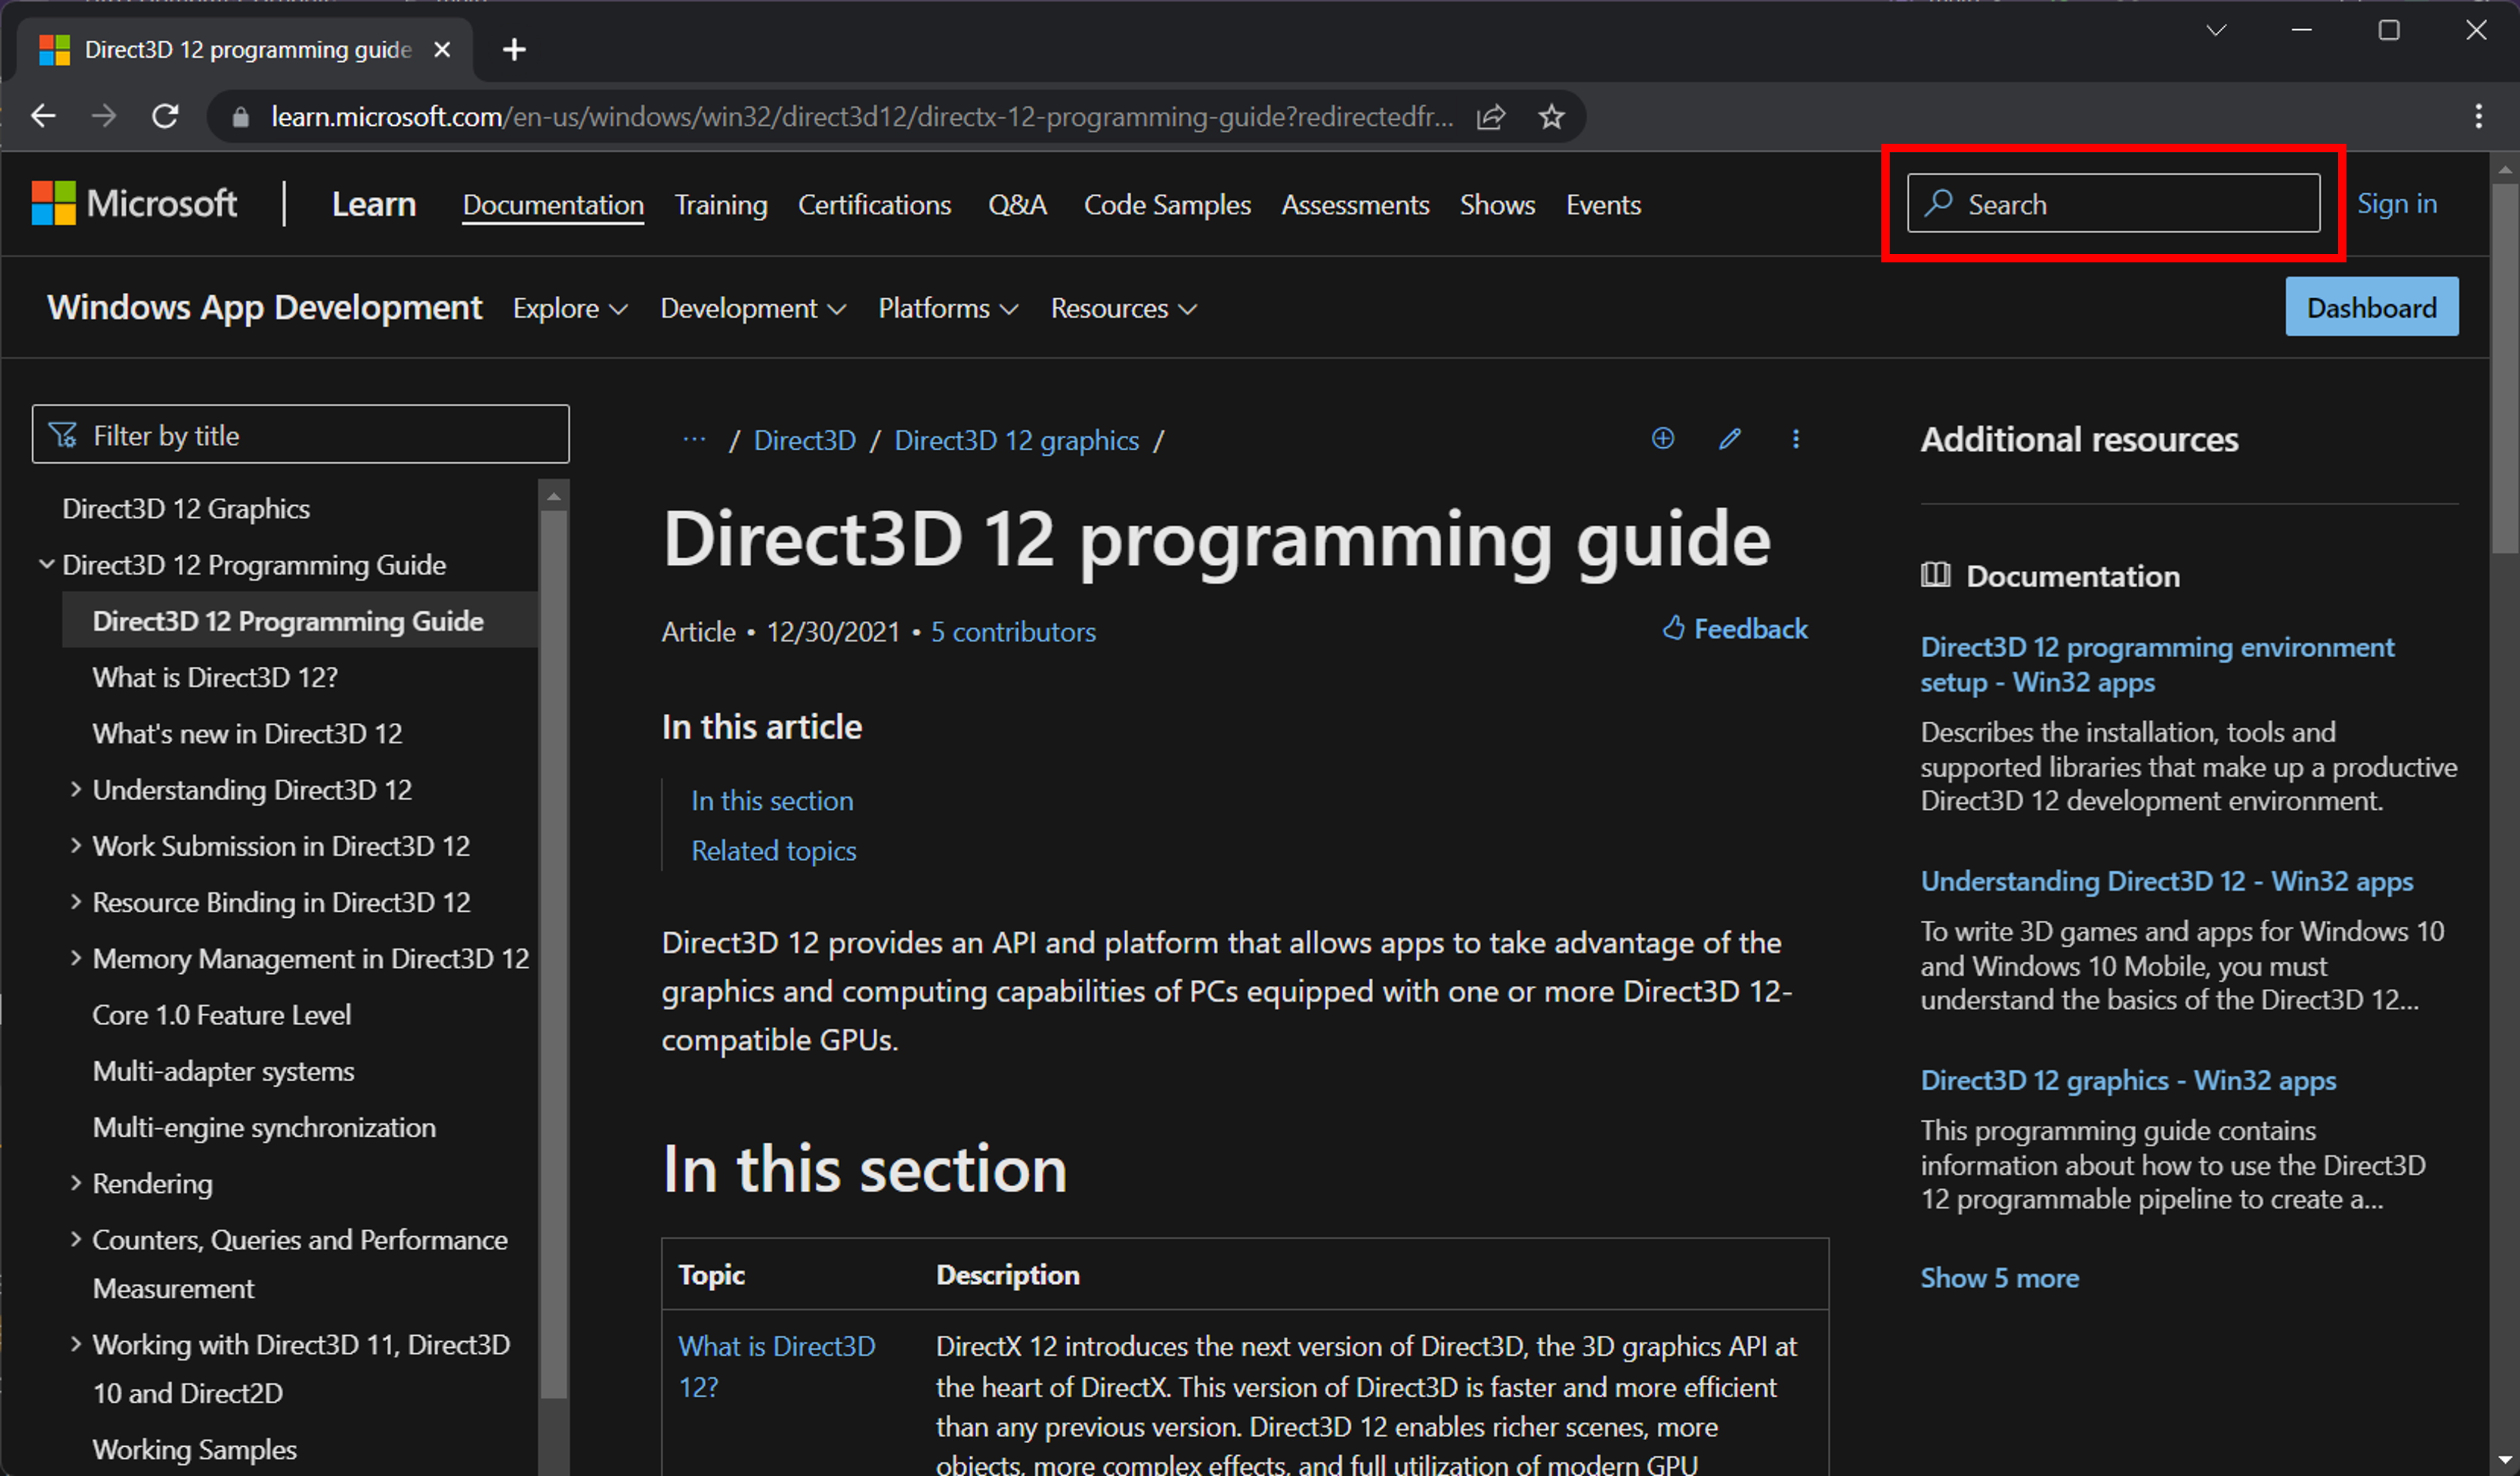
\includegraphics[width=\textwidth]{Images/1.Intro.1.1.png}
        \caption{راهنمای برنامه نویسی \lr{Direct3D} در مستندات \lr{DirectX}.}
        \\[20pt]
        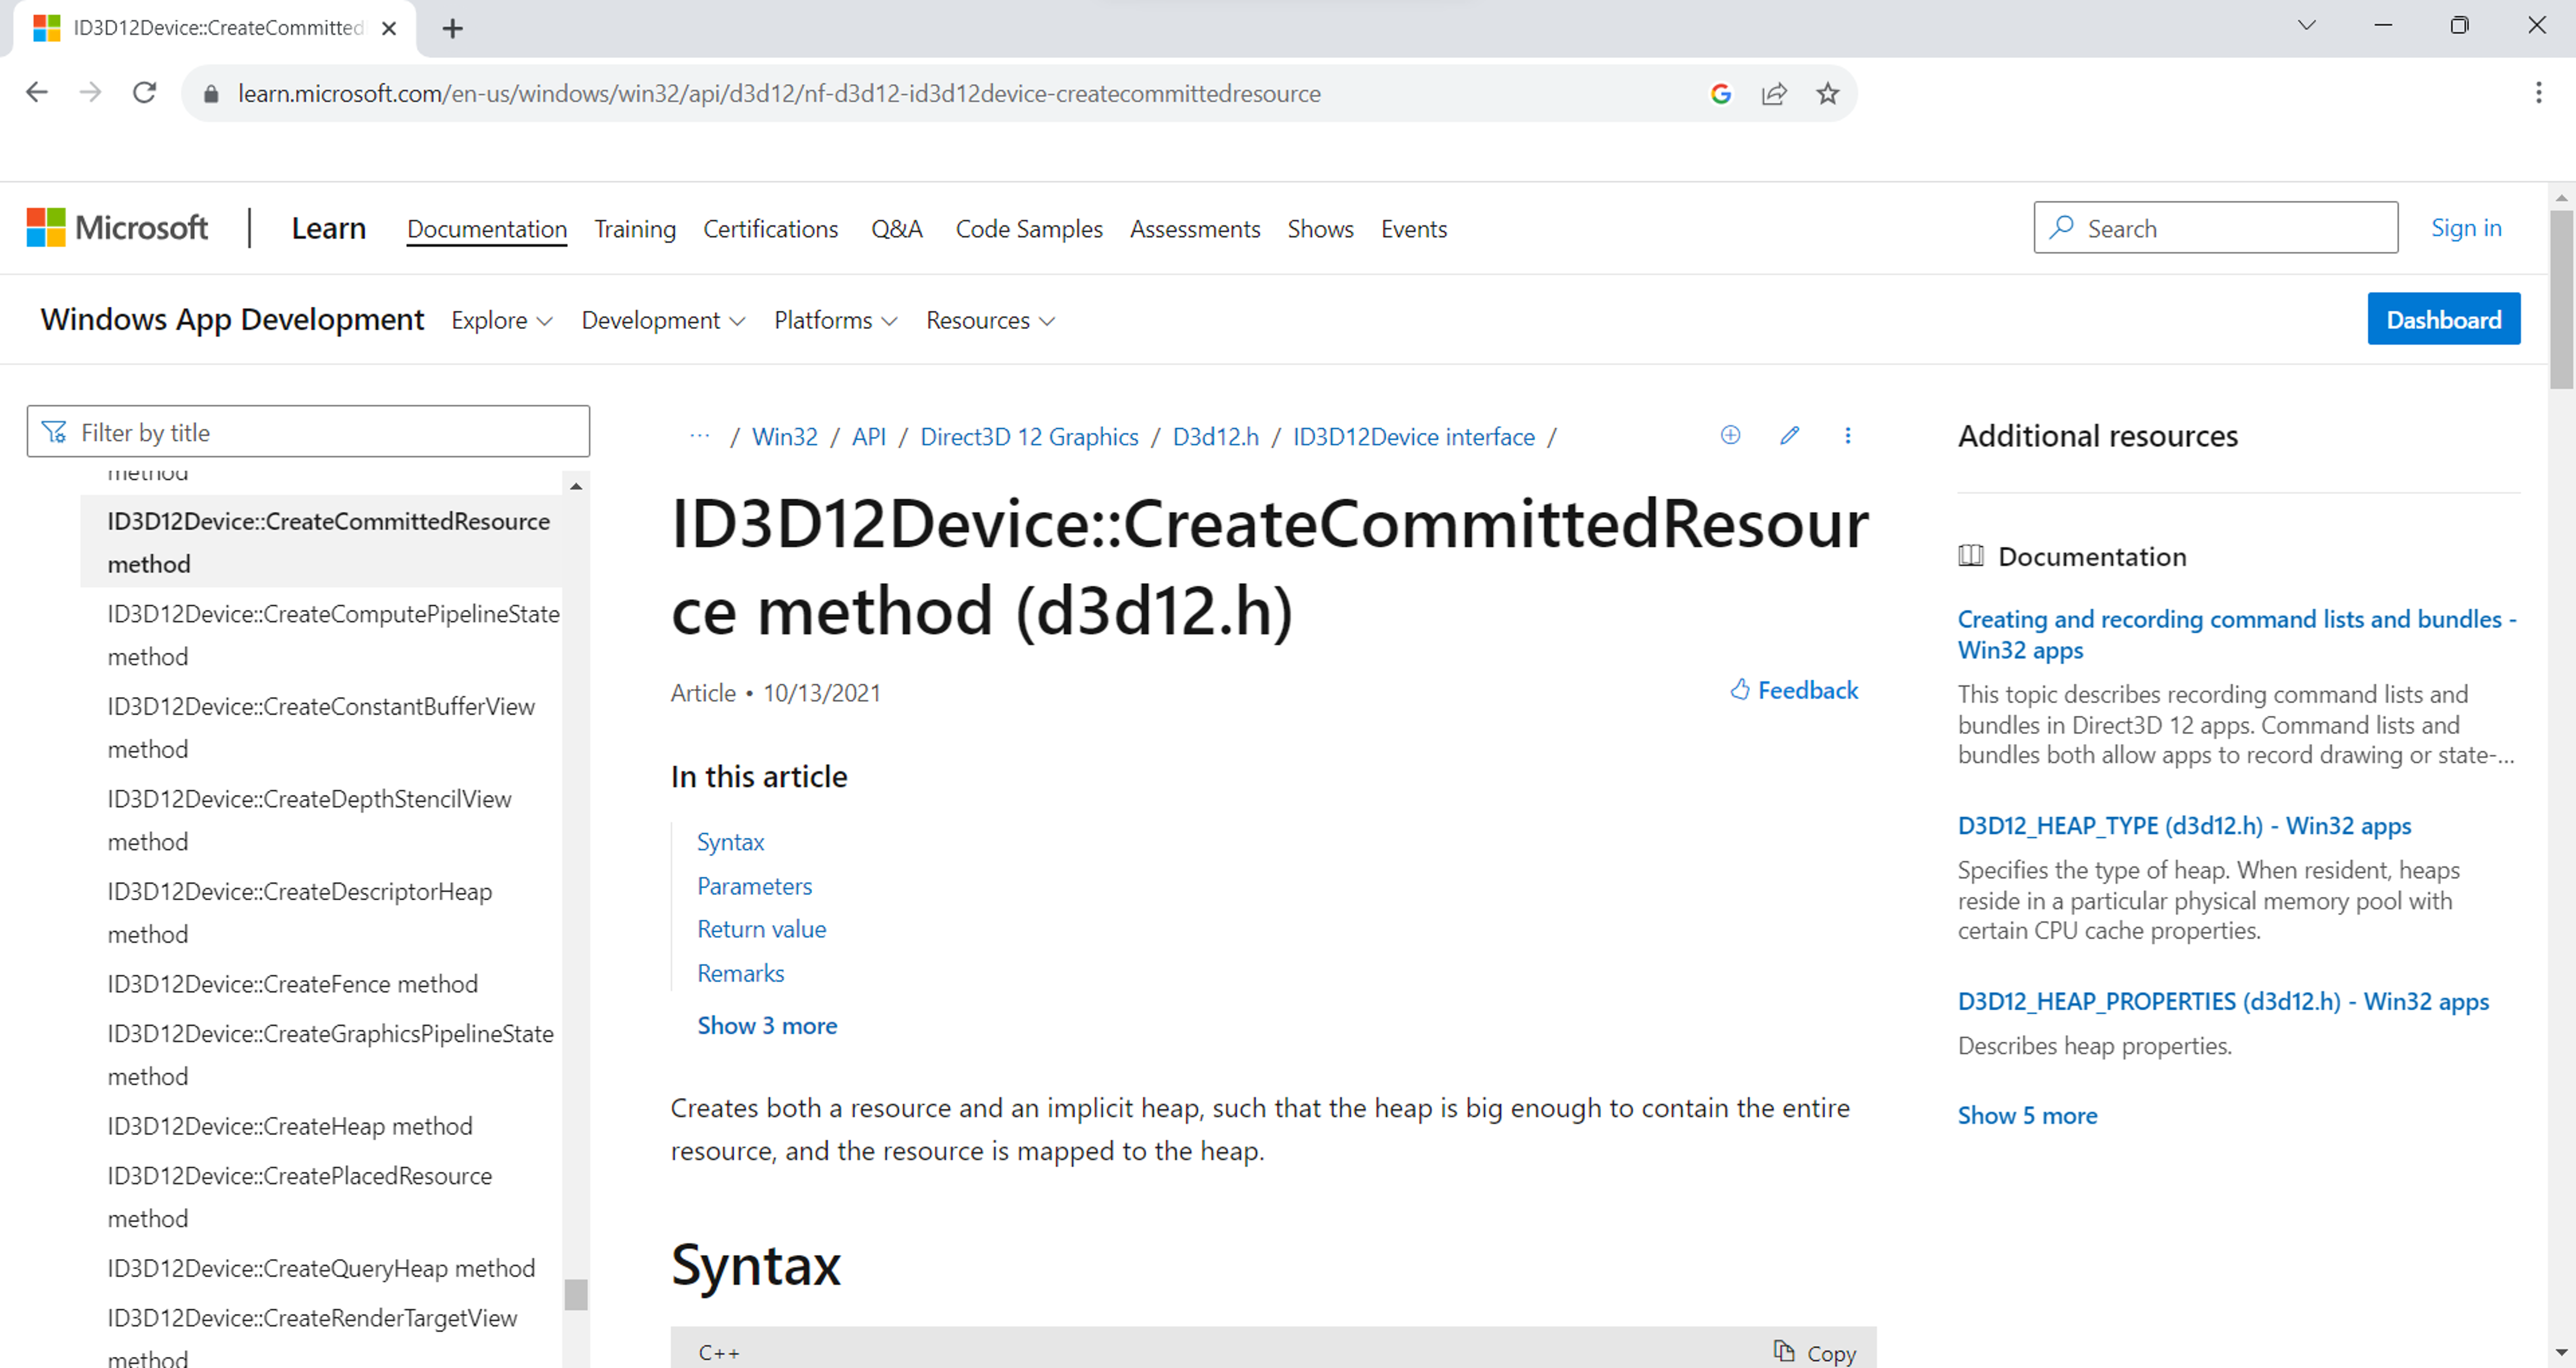
\includegraphics[width=\textwidth]{Images/1.Intro.1.2.png}
        \caption{دریافت مستندات یک تابع.}
    \end{figure}

    \begin{theo}{thm:pythagoras}
        در این کتاب ممکن است هر از گاهی برای جزئیات بیشتر شما را به مستندات راهنمایی کنیم.
    \end{theo}
    ما همچنین می خواهیم به برنامه های نمونه \lr{Direct3D 12} که به صورت آنلاین در دسترس هستند اشاره کنیم:

    \begin{flushleft}
        \href{https://github.com/Microsoft/DirectX-Graphics-Samples}{https://github.com/Microsoft/DirectX-Graphics-Samples}
    \end{flushleft}

    نمونه‌های بیشتری در آینده خواهند آمد و همچنین به میتوانید نمونه‌های \lr{Direct3D 12} را در وب‌سایت‌های \lr{NVIDIA}، \lr{AMD} و \lr{Intel} مشاهده کنید.
} %\\[20pt]
\textbf{\vspace{25pt}}

\title{
    \LARGE
    \textbf{شفاف سازی}
} \rullFillWithLine[0.5em]{1pt}
\textbf{\vspace{12pt}}

{
    \Large
    اگرچه ما در تلاش برای نوشتن کد کارآمد و پیروی از بهترین شیوه های برنامه نویسی \lr{Direct3D 12} هستیم، اما هدف اصلی هر برنامه ی نمونه ، نشان دادن مفاهیم \lr{Direct3D} یا تکنیک های برنامه نویسی گرافیکی است.
    نوشتن بهینه‌ترین کد هدف نبود و احتمالاً ایده‌هایی را که تلاش می‌کردند به تصویر کشیده شوند را مبهم می‌کرد.
    اگر از کد نمونه در پروژه های خود استفاده می کنید، این را در نظر داشته باشید، زیرا ممکن است بخواهید برای کارایی بهتر دوباره روی آن کار کنید.
    علاوه بر این، به منظور تمرکز بر \lr{Direct3D API}، زیرساخت های حداقلی را در بالای \lr{Direct3D} ایجاد کرده ایم. این بدان معنی است که ما مقادیر هاردکد را تعیین کردیم و چیزهایی را در کد منبع تعریف می کنیم که معمولاً ممکن است مبتنی بر داده باشند.
    در یک برنامه بزرگ سه بعدی، احتمالاً یک موتور رندر در بالای \lr{Direct3D} پیاده سازی خواهید کرد. با این حال، موضوع این کتاب \lr{Direct3D API} است، نه طراحی موتور رندر.
}
\textbf{\vspace{25pt}}

\title{
    \LARGE
    \textbf{نمونه برنامه ها و مکمل های آنلاین}
} \rullFillWithLine[0.5em]{1pt}
\textbf{\vspace{12pt}}

{
    \Large
    وب‌سایت این کتاب (\href{www.d3dcoder.net}{www.d3dcoder.net} و \href{www.merclearning.com}{www.merclearning.com}) نقش مهمی در استفاده حداکثری از این کتاب دارد.
در وب سایت شما کد منبع کامل و فایل های پروژه را برای هر نمونه در این کتاب خواهید یافت.
در بسیاری از موارد، برنامه های \lr{DirectX} آنقدر بزرگ هستند که نمی توانند به طور کامل در یک کتاب درسی جاسازی شوند. بنابراین، ما فقط قطعات کد مربوطه را بر اساس ایده‌هایی که نشان داده می‌شوند جاسازی می‌کنیم.
اکیداً توصیه می شود که خواننده کد آزمایشی مربوطه را مطالعه کند تا برنامه را به طور کامل ببیند. (هدف ما این است که دموها را برای مطالعه آسان کوچک و متمرکز کنیم.) به عنوان یک قاعده کلی، خواننده باید بتواند پس از خواندن فصل و گذراندن مدتی برای مطالعه کد نسخه ی نمایشی، نسخه ی نمایشی (های) فصل را به تنهایی پیاده سازی کند.
در واقع یک تمرین خوب این است که سعی کنید نمونه ها را خودتان با استفاده از کتاب و کد نمونه به عنوان مرجع پیاده سازی کنید.
}
\textbf{\vspace{25pt}}

\title{
    \LARGE
    \textbf{راه اندازی پروژه آزمایشی در \lr{Visual Studio 2022}}
} \rullFillWithLine[0.5em]{1pt}
\textbf{\vspace{12pt}}

{
    \Large
    دموهای این کتاب را می توان به سادگی با دوبار کلیک کردن روی فایل پروژه مربوطه \lr{(.vcxproj)} یا فایل \lr{solution (sln.)} باز کرد.
    این بخش نحوه ایجاد و ساخت یک پروژه را از ابتدا با استفاده از چارچوب برنامه آزمایشی کتاب با استفاده از \lr{Visual Studio 2022} توضیح می‌دهد.
    به عنوان یک مثال کاربردی، نحوه بازآفرینی و ساخت نسخه نمایشی \lr{"Box"} از فصل 6 را نشان خواهیم داد.
}
\textbf{\vspace{25pt}}

\title{
    \Large
    \rullCenterTextWithLine{\textbf{کد منبع کتاب را دانلود کنید}}
}
\textbf{\vspace{12pt}}

{
    \Large
    ابتدا کد منبع کتاب را در پوشه ای در هارد دیسک خود دانلود کنید.
    برای بحث، فرض می کنیم این پوشه \grayBox{\lr{C:\symbol{92}d3d12book}} است.
    در پوشه کد منبع، فهرستی از پوشه‌ها را برای هر فصل خواهید دید. هر پوشه شامل پروژه های کد برای فصل داده شده است.
    همچنین به پوشه ای به نام \lr{Common} توجه کنید. این پوشه حاوی کد منبع به اشتراک گذاشته شده است که در تمام پروژه های آزمایشی استفاده مجدد می شود.
    اکنون، در پوشه کد منبع، یک پوشه جدید ایجاد کنید که می خواهید دموهای خود را در آن ذخیره کنید. برای مثال، \grayBox{\lr{C:\symbol{92}d3d12book\symbol{92}MyDemos}}. این پوشه جایی است که می توانید پروژه های جدید را بر اساس چارچوب نمونه کتاب ایجاد کنید.
}
{
    \Large
    این ساختار دایرکتوری کاملاً ضروری نیست، اما ساختاری است که دموهای کتاب از آن پیروی می کنند. اگر با تنظیم مسیرهای شامل اضافی راحت هستید، می‌توانید پروژه‌های نمایشی خود را در هر مکانی قرار دهید تا زمانی که به \lr{Visual Studio} راهنمایی کنید که چگونه کد منبع را در فهرست مشترک پیدا کند.
}
\textbf{\vspace{25pt}}

\title{
    \Large
    \rullCenterTextWithLine{\textbf{موارد مورد نیاز \lr{Visual Studio} را نصب کنید}}
}
\textbf{\vspace{12pt}}

{
    \Large
    ابتدا \lr{Visual Studio Installer} را باز کنید. از پنجره ی باز شده ، \lr{Modify} یا \lr{Install} را کلیک کنید. در سمت چپ پنجره ی باز شده ، از قسمت \lr{\grayBox{Desktop \& Mobile}} ، تیک قسمت های \lr{Universal Windows Platform development} و \lr{Desktop development with C++} را بزنید.
    از قسمت \lr{\grayBox{Gaming}} نیز تیک \lr{Game development with C++} را بزنید.

    \begin{figure}[H]
        \centering
        \setlength{\belowcaptionskip}{-10pt}
        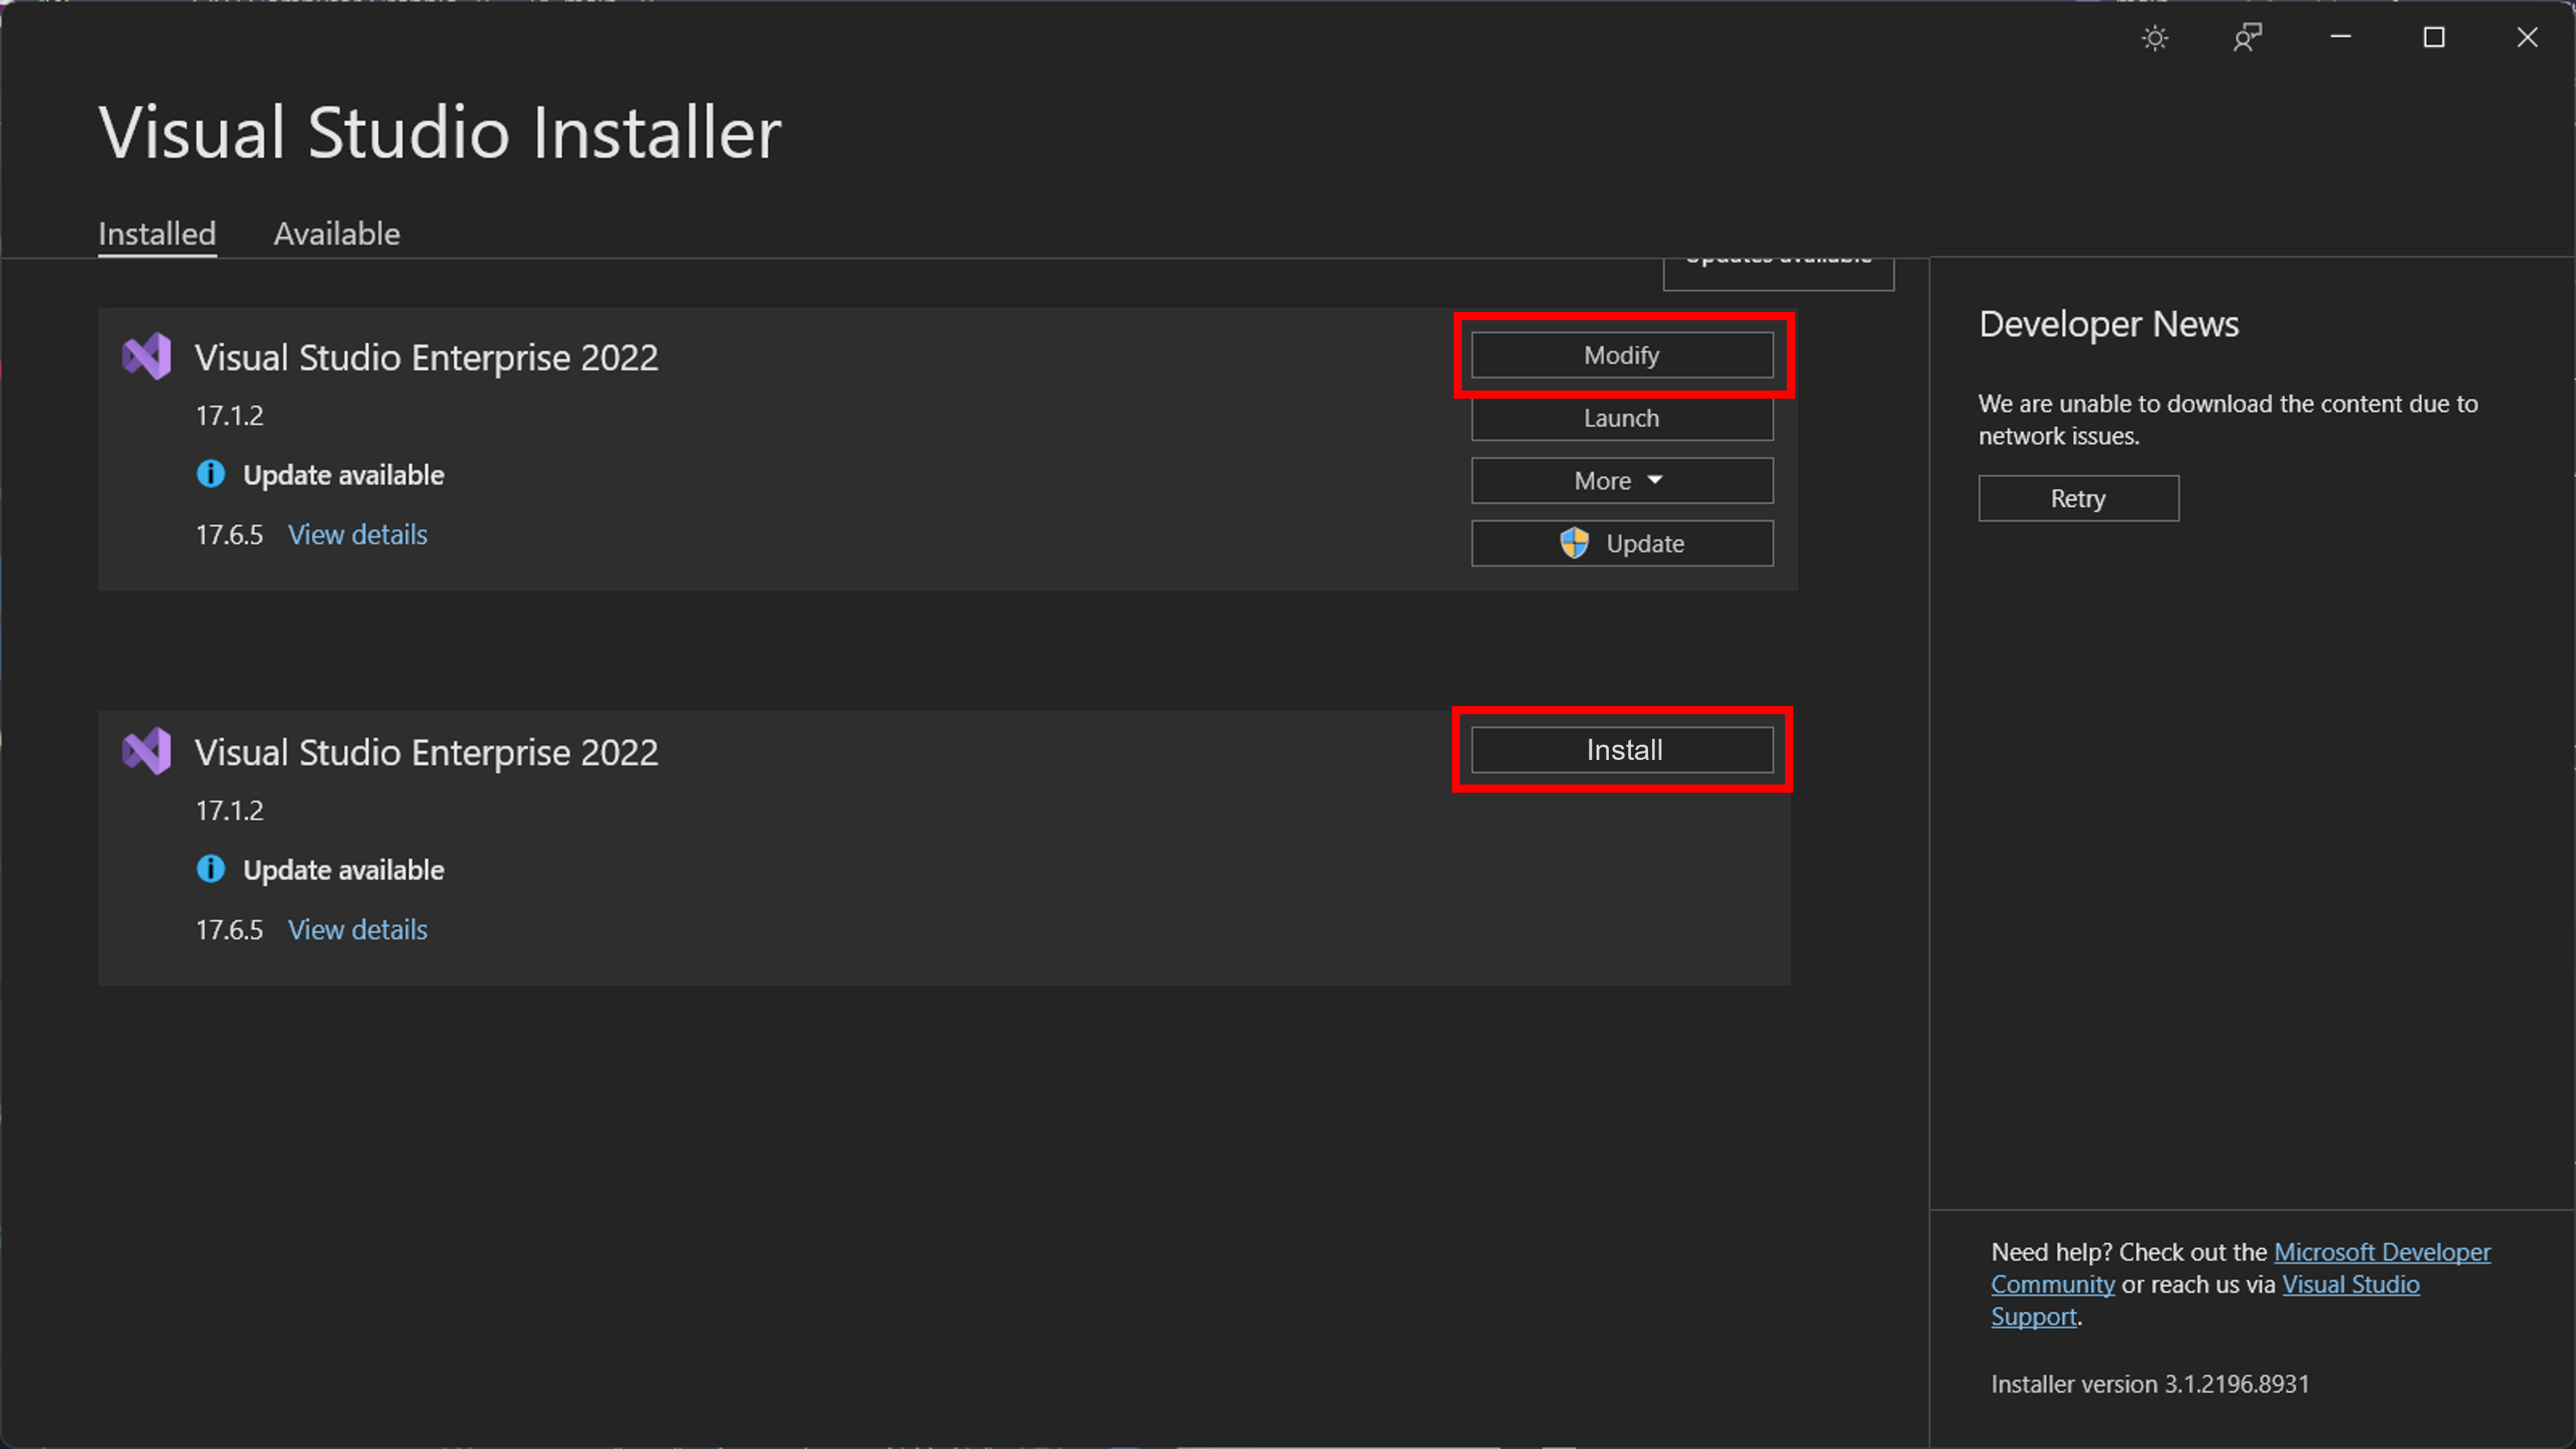
\includegraphics[width=\textwidth]{Images/1.Intro.2.1.png}
        \caption{محیط \lr{Visual Studio Installer}.}
        \\[20pt]
        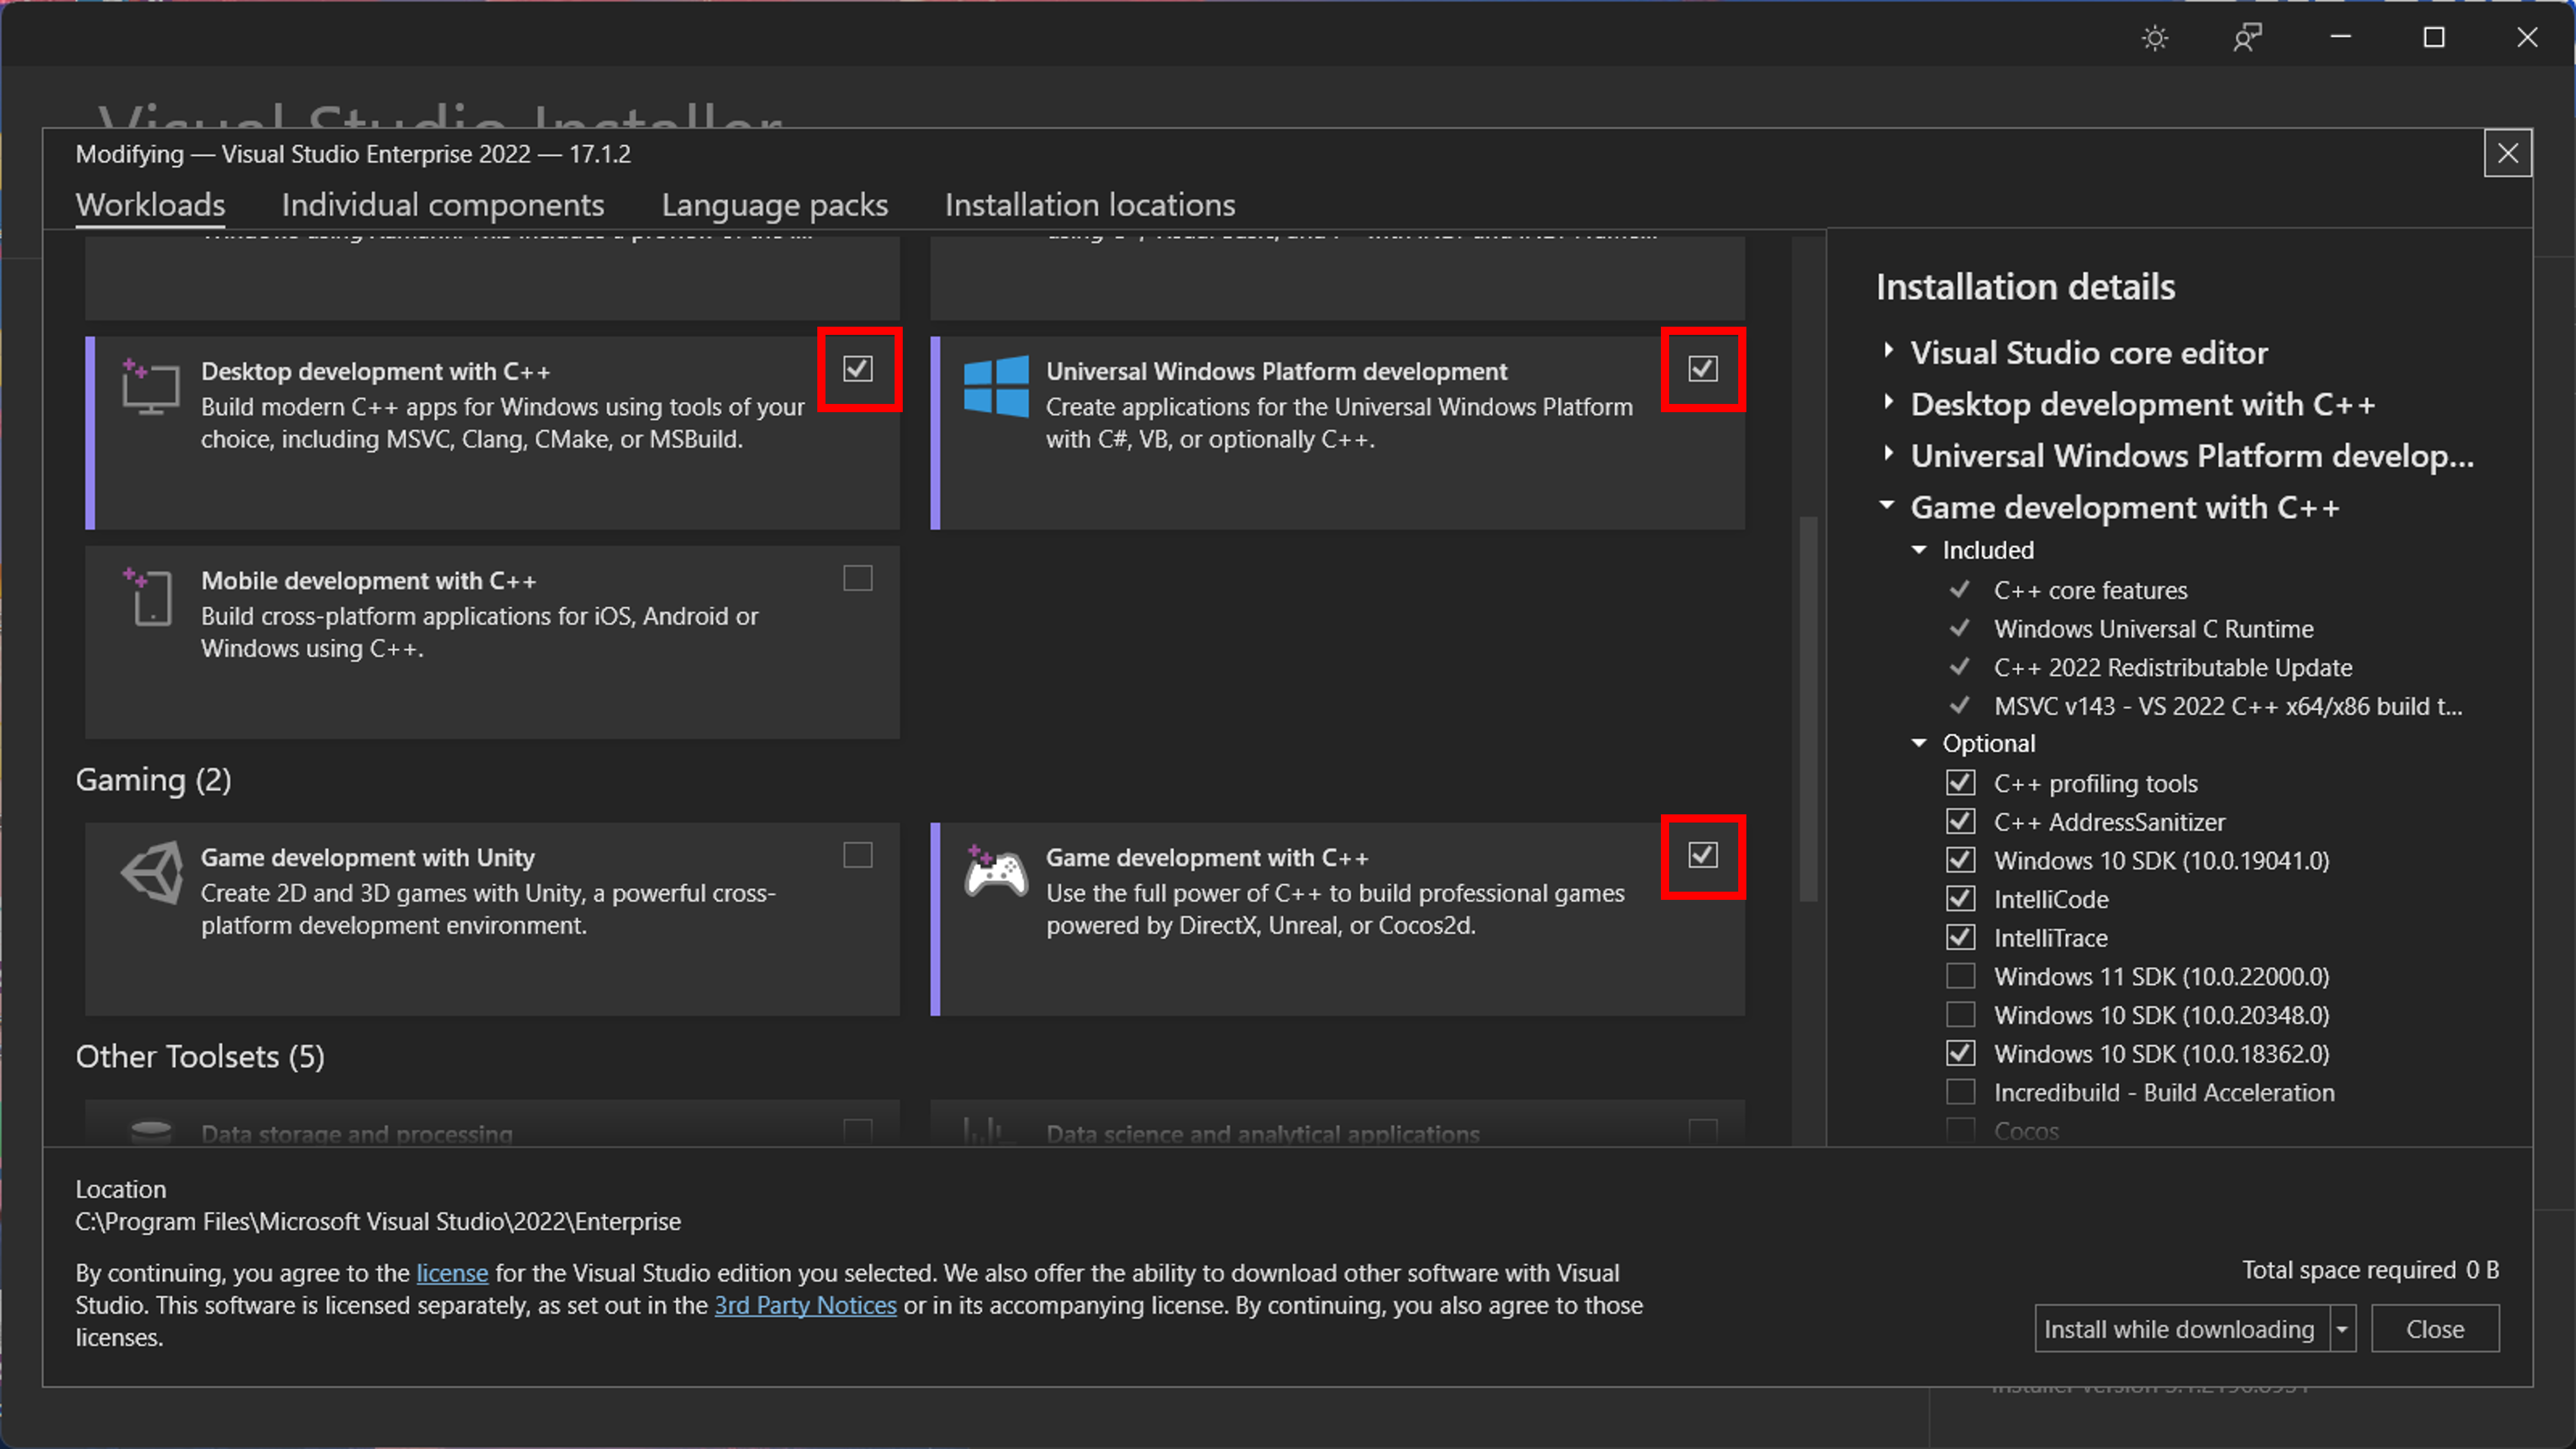
\includegraphics[width=\textwidth]{Images/1.Intro.2.2.png}
        \caption{مواردی که باید نصب شوند.}
    \end{figure}

    بعد از نصب موارد بالا ، باید از نصب موارد اضافه تری نیز مطمئن شوید. این موارد شامل \lr{SDK} های ویندوز و ورژن های جدید \lr{C++} است.
    در سمت راست پنجره ی باز شده ، میتوانید این موارد را ببینید. برای اجرای بهتر ، سعی کنید موارد را مانند عکس ها رعایت کنید.

    \begin{figure}[H]
        \centering
        \setlength{\belowcaptionskip}{-10pt}
        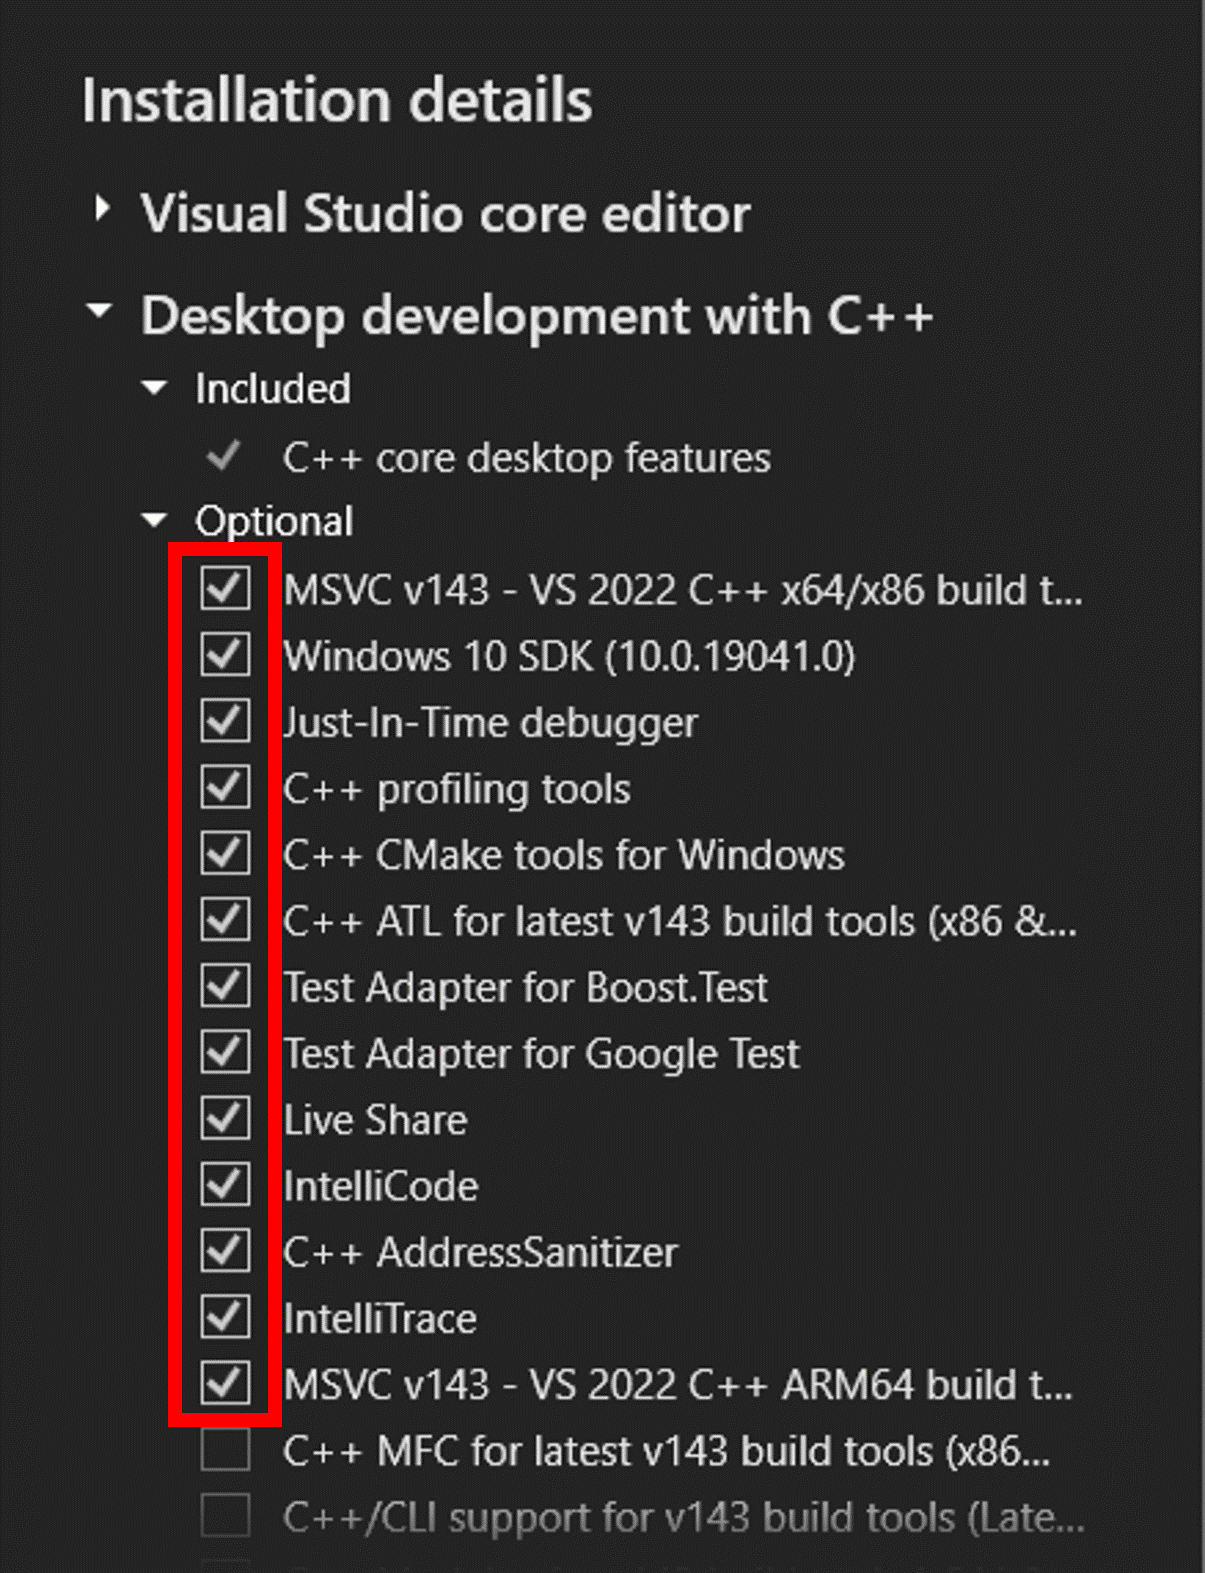
\includegraphics[scale=0.7]{Images/1.Intro.3.1.png} \hspace{5mm}
        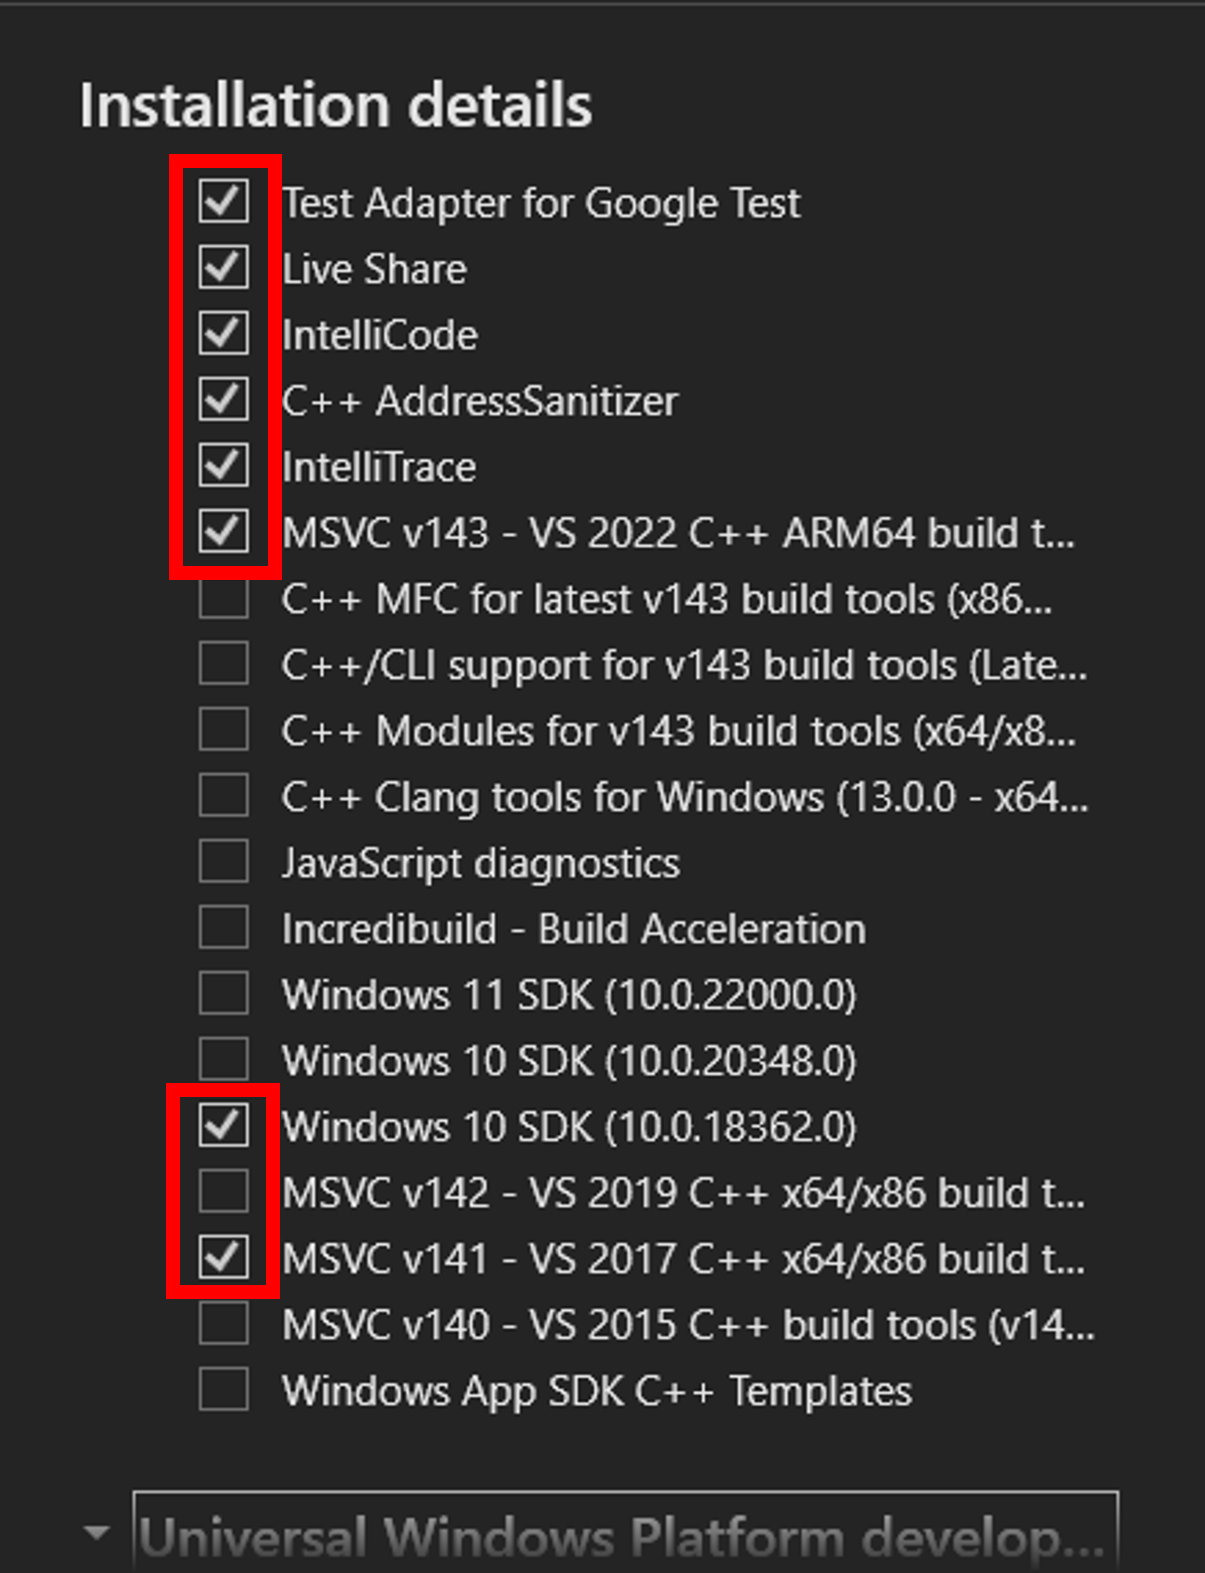
\includegraphics[scale=0.7]{Images/1.Intro.3.2.png}
        \\[25pt]
        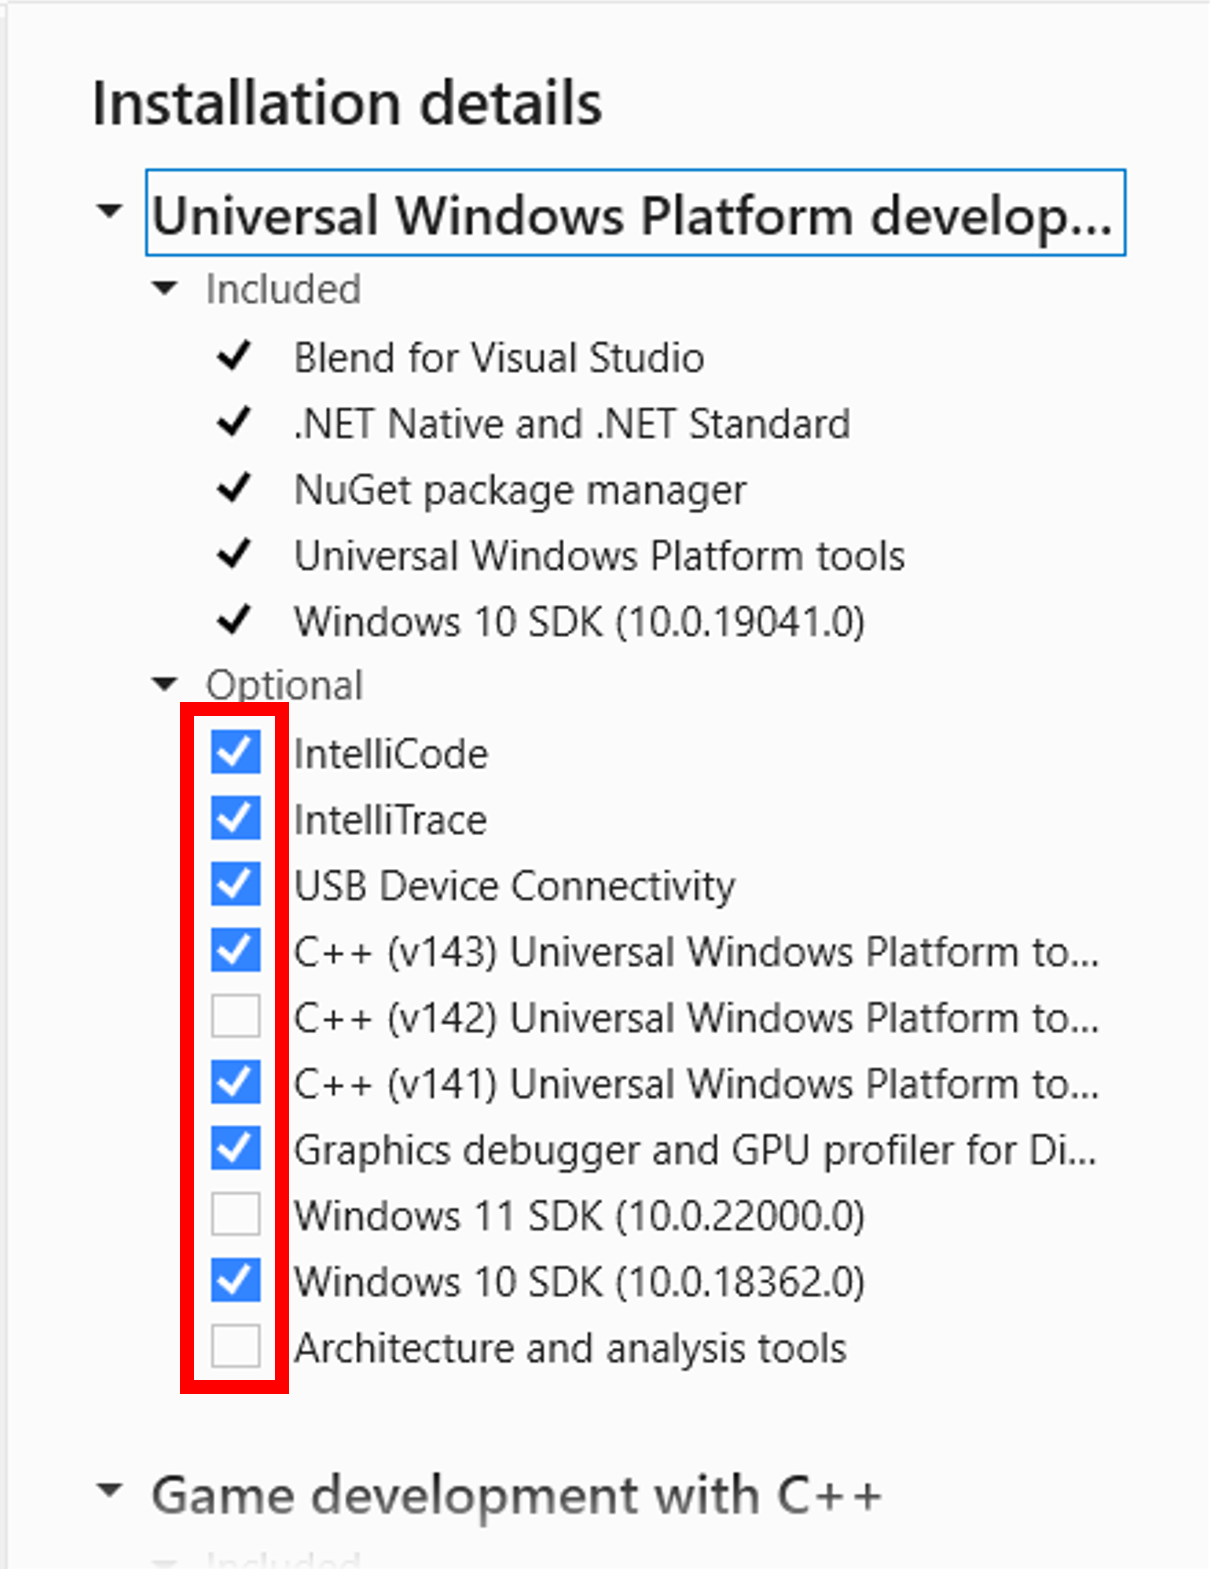
\includegraphics[scale=0.7]{Images/1.Intro.3.3.png} \hspace{5mm}
        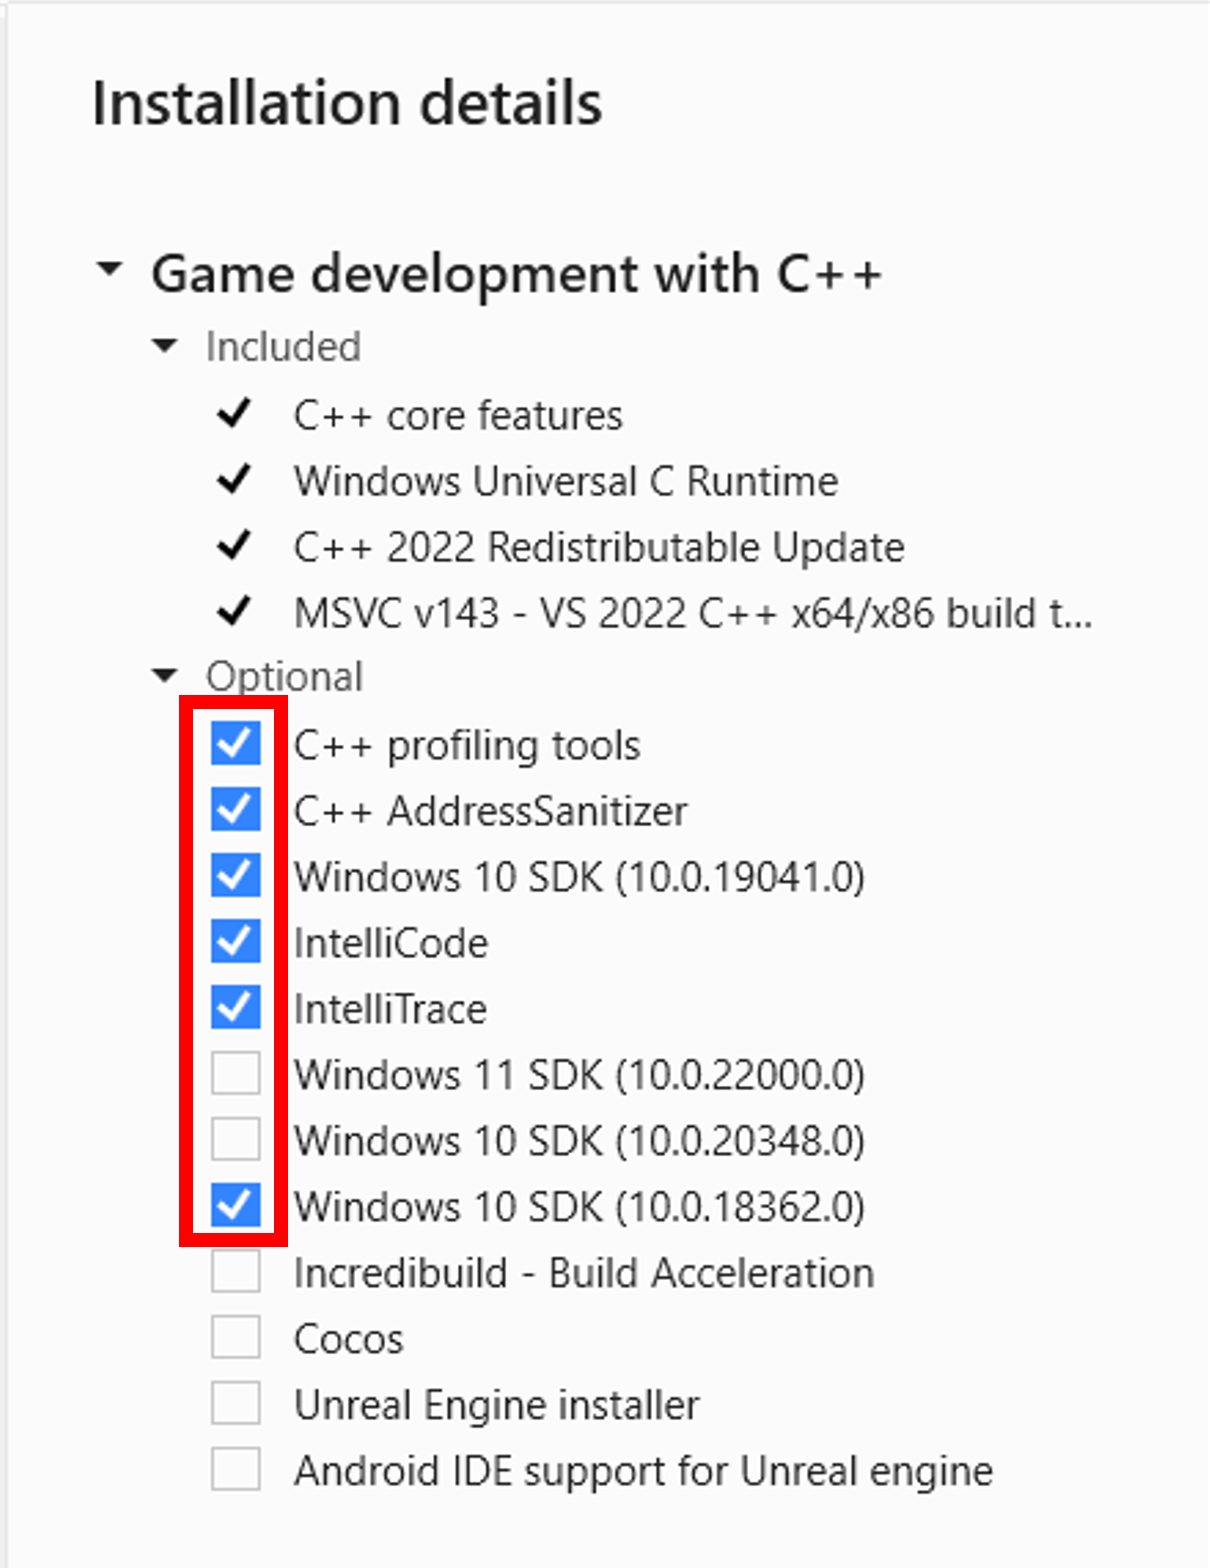
\includegraphics[scale=0.7]{Images/1.Intro.3.4.png}
        \caption{مواردی که باید نصب شوند.}
    \end{figure}
}
\textbf{\vspace{12pt}}

\title{
    \Large
    \rullCenterTextWithLine{\textbf{فعال کردن \lr{Graphic Tools}}}
}
\textbf{\vspace{14pt}}

{
    \Large
    برای اجرای درست برنامه های دموی \lr{DirectX 12} ، نیاز است که قابلیت \lr{Graphic Tools} در ویندوز شما فعال باشد.
    برای این کار میتوانید به صورت عمل کنید.

    \textbf{روش اول)}
    ابتدا در منوی استارت ، \lr{Optional features} را سرچ کرده و آن را باز کنید.
    اگر \lr{Graphic Tools} از قبل بر روی دستگاه شما نصب شده باشد ، میتوانید از قسمت پایین پنجره آن را مشاهده کنید.
    در غیر این صورت بر روی \lr{\grayBox{View features}} کلیک کرده و نام آن را سرچ کرده و نصب کنید.

    \begin{figure}[H]
        \centering
        \setlength{\belowcaptionskip}{-10pt}
        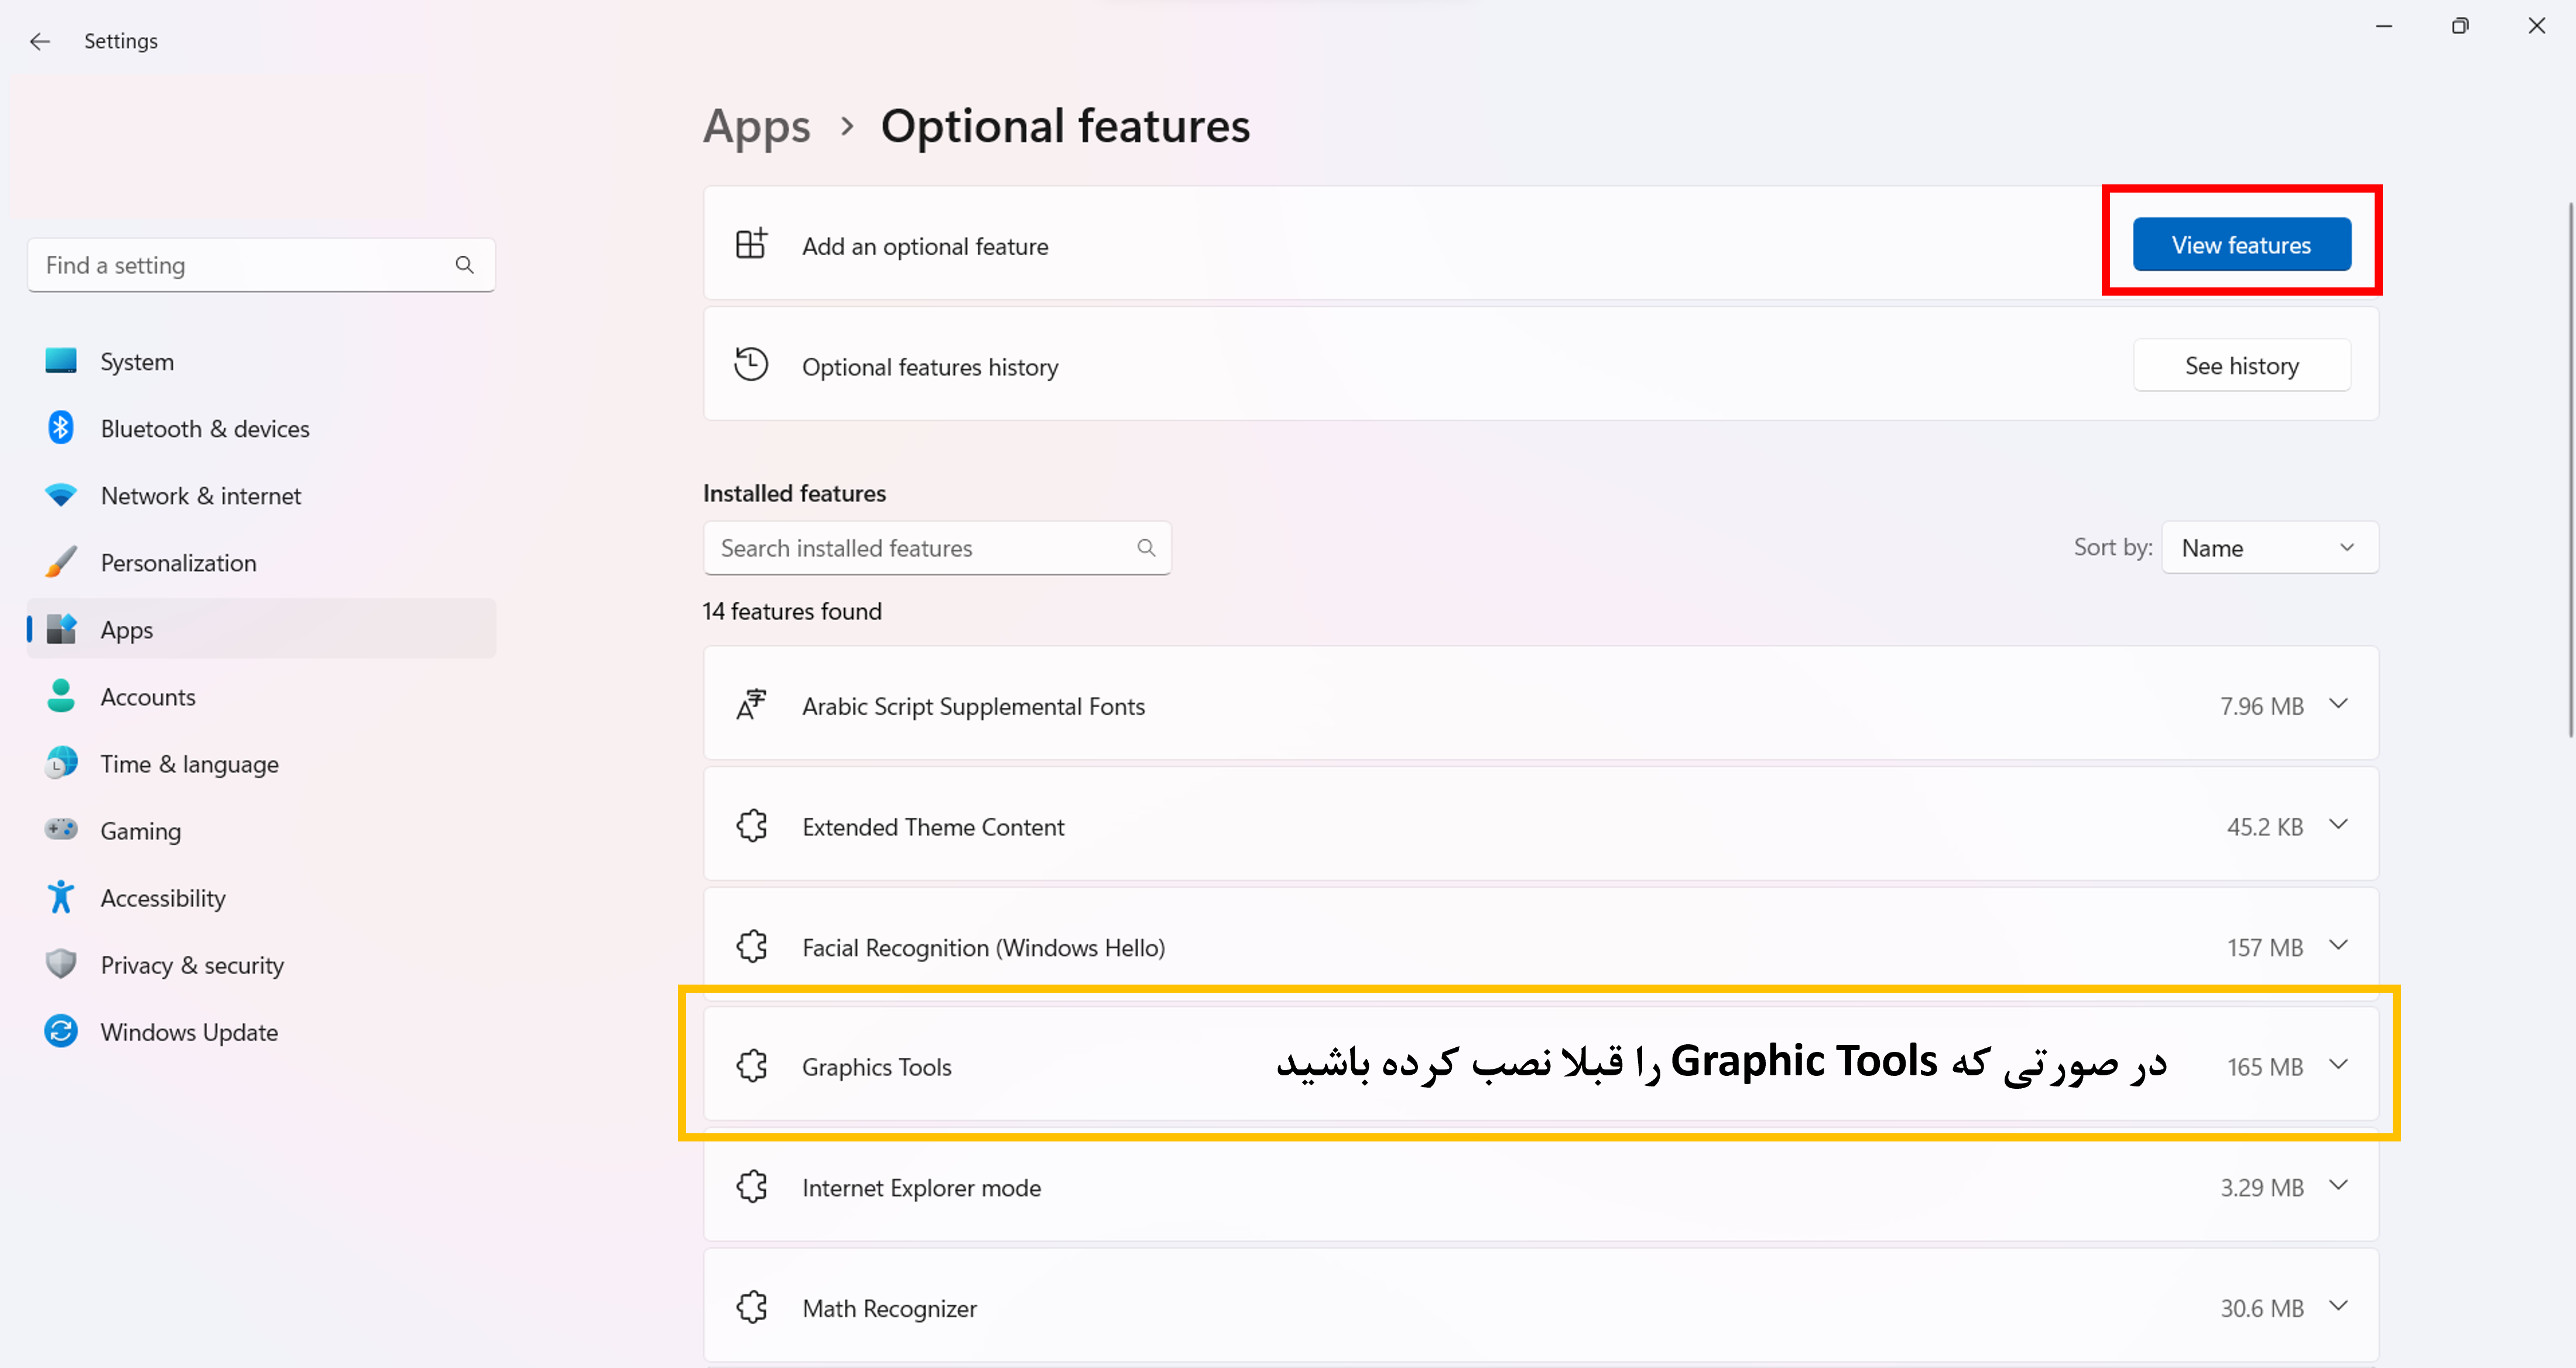
\includegraphics[width=\textwidth]{Images/1.Intro.4.1.png}
        \caption{محیط \lr{Optional features}.}
    \end{figure}

    \textbf{روش دوم)}
    اگر به هر دلیلی روش اول برای شما قابل انجام نبود ، میتوانید پنجره ی \lr{Command Prompt} (\lr{CMD}) را باز کرده و با دستورات زیر آن را نصب کنید.

    ابتدا دستور داخل \lr{CMD} عبارت زیر را وارد کنید:

    \begin{flushleft}
        \grayBox{Dism /Online /Get-Packages /Format:Table}
    \end{flushleft}

    از لیست نشان داده شده ، موردی را که با \lr{\grayBox{Tools.Graphics.DirectX}} شروع میشود را پیدا کرده و کامل نام آن را کپی کنید. (ممکن است اعداد مقابل آن با عکس متفاوت باشد)

    سپس دستور زیر را وارد کنید و به جای \lr{\grayBox{<Name>}} ، نامی که کپی کردید را قرار دهید.

    \begin{flushleft}
        \grayBox{Dism /Online /Add-Capability /CapabilityName:<Name>}
    \end{flushleft}

    به عنوان مثال:

    \begin{flushleft}
        \normalsize
        \grayBox{Dism /Online /Add-Capability /CapabilityName:Tools.Graphics.DirectX\textasciitilde\textasciitilde\textasciitilde\textasciitilde0.0.1.0}
    \end{flushleft}
}
\textbf{\vspace{25pt}}

\begin{theo}{thm:pythagoras}
{
    \Large
    دقت کنید که فرآیند نصب ممکن است زمان بر باشد. همچنین دستورات \lr{Dism} به بزرگ و کوچک بودن حروف حساس نیستند.
}
\end{theo}

%--------------------------------------%
\newpage